% !TeX spellcheck = de_CH_frami
\section{Stand der Arbeit}
\subsection{Plan}
\frame{\frametitle{Plan}
	\begin{center}
		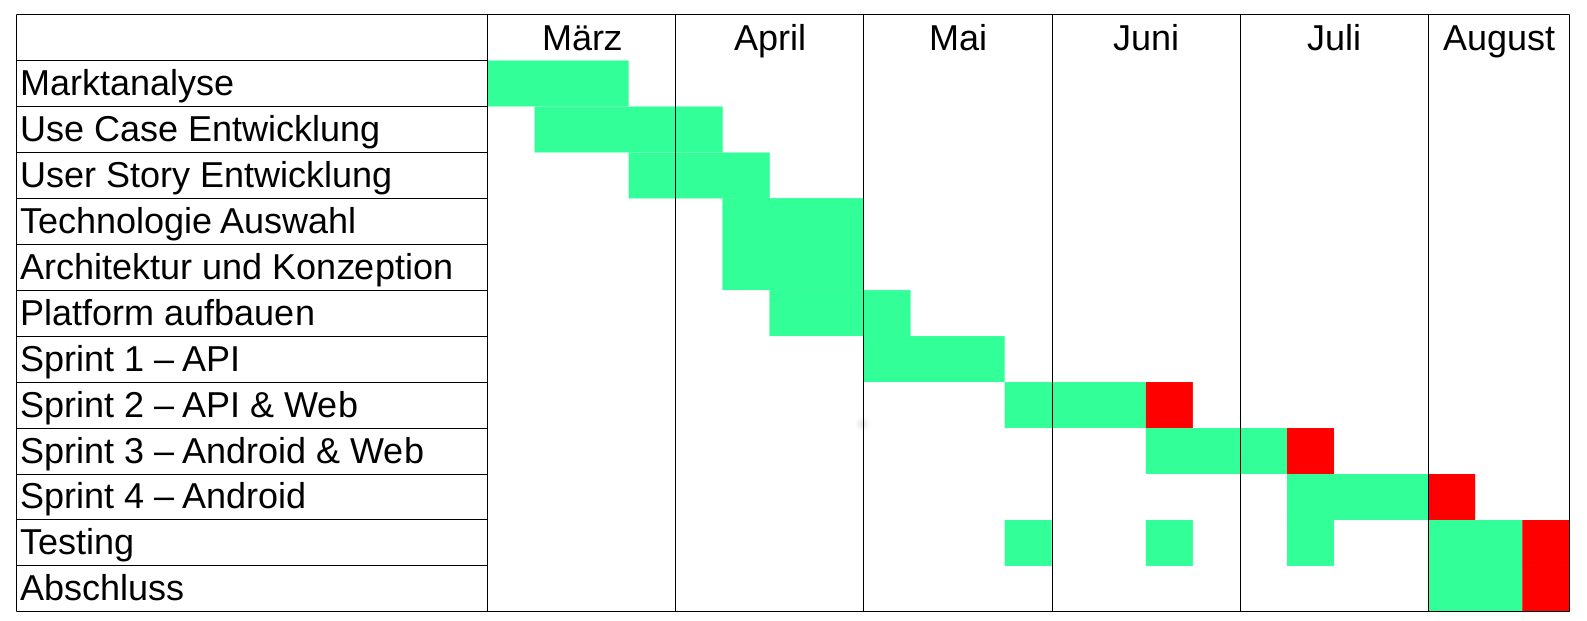
\includegraphics[scale=0.2]{pic/Grobplanung.png}
	\end{center}
}
\subsection{Dokumentation}
\frame{\frametitle{Stand der Arbeit}

\begin{itemize}
\item Use Cases und Anforderungen definiert (braucht noch �berarbeitung)
\item User Stories gr�sstenteils definiert - braucht cleanup

\item Konzepte und Technologien dokumentiert (braucht noch �berarbeitung)
\item Workflows Dokumentiert

\end{itemize}


}

\frame{\frametitle{Arbeitsprodukte - API und Web}
	
	
	\begin{itemize}
		\item API Programmiert, Alpha Status
		\item Website Programmiert - Alpha Status
		\item Funtionalit�ten nach Aufgabenstellung \grqq rudiment�r\grqq  umgesetzt
		\end{itemize}
		
		
	}
	\frame{\frametitle{Android App}
		
		
		\begin{itemize}
			\item keine native Androdi App vorhanden
			\item APK generiert f�r Website
			\item Konzept f�r Push Nachrichten trotz WEB-APK
		\end{itemize}}
		
		